\chapter{Le vélo}
\section*{29 octobre 2014}
Mon objectif est de faire une bonne partie des déplacements en vélo, il me faut donc un vélo adapté au voyage : \newline
 – Solide et fiable \newline
 – Réparable, donc avec des pièces standards \newline
 – Adapté à la route et aux chemins \newline
 – A un prix raisonnable \newline
 Les contacts que j'ai eu avec les vendeurs de vélos ne m'ont pas convaincu d'acheter un vélo tout prêt, ni d'en faire monter un sur mesure : prix élevés, configuration du vélo trop haut de gamme ou peu adapté. \newline
 J'ai choisi de monter le vélo en achetant toutes les pièces séparément, ce qui a l'avantage de me donner une bonne connaissance du vélo et du montage. Cela sera sans doute utile à un moment ou à un autre. \newline
 J'ai d'abord acheté un VTT d'occasion datant de 1992, principalement à cause du cadre en acier Tange, solide et réparable. En plus, j'ai gardé certaines autres pièces. \newline
 \newline
\centerline{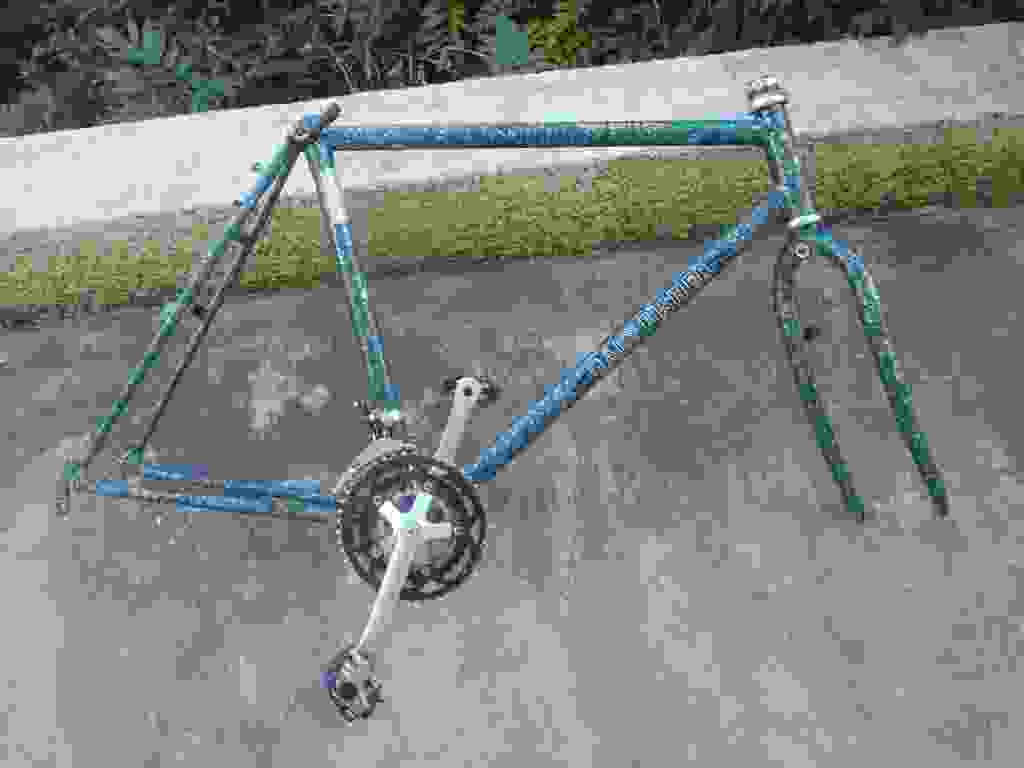
\includegraphics[width=\mywidth]{../wp-content/uploads/2014/10/Cadre.jpg} } 
 \newline
 J'ai ensuite monté des pièces neuves, que j'ai choisies en m'appuyant sur les conseils que j'ai trouvés sur les blogs ou les forums. \newline
 Et le résultat : \newline
 \newline
\centerline{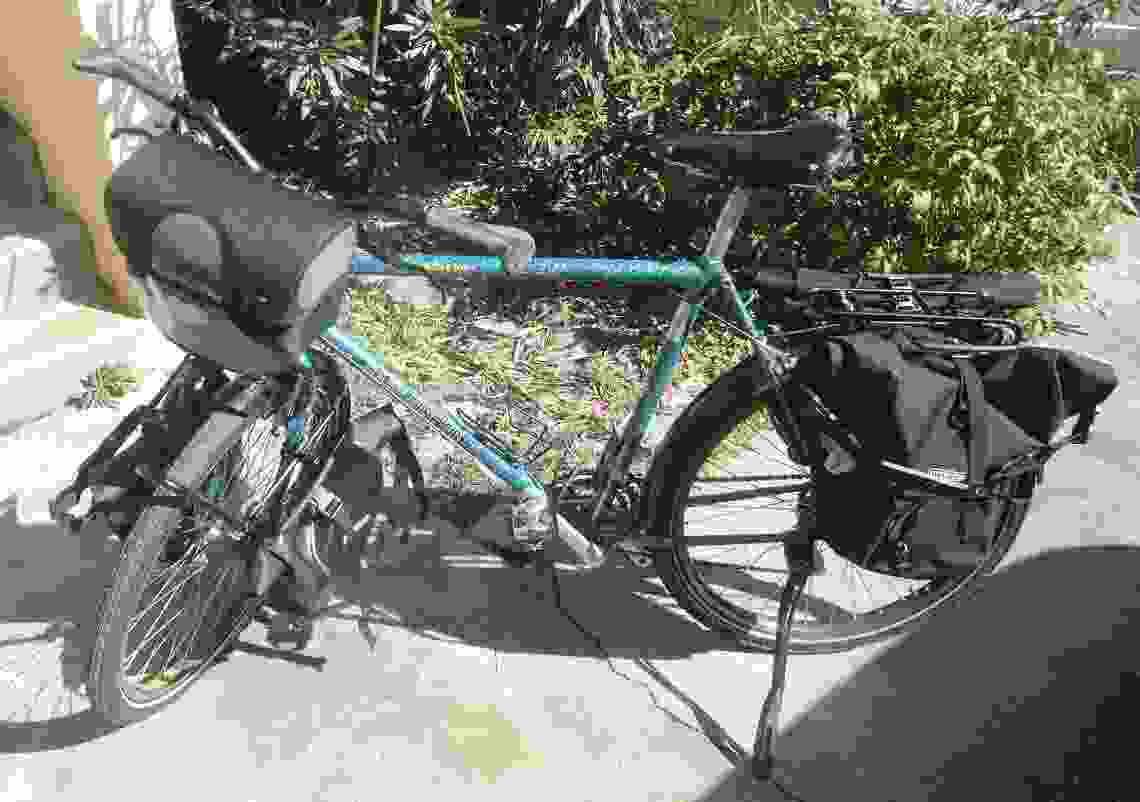
\includegraphics[width=\mywidth]{../wp-content/uploads/2014/10/Velo.jpg} } 
 \newline
 Ça donne un vélo complet pour environ 1000€, sacoches comprises. Voici le détail de la composition du vélo : \newline
  \begin{tabular}{|l|l|}
\hline     Elément &  Modèle    \\ 
 \hline 
  Cadre + fourche &  Gary Fisher (acier tange)    \\ 
 \hline 
  Jeu de direction &  D'origine du VTT    \\ 
 \hline 
  Potence + plongeur &  BBB Highrise 110mm    \\ 
 \hline 
  Cintre &  relevé XLC 63cm    \\ 
 \hline 
  Poignées &  Ergonomique avec Bar End intégrés   \\ 
 \hline 
  Transmission AV &  Shimano Deore LX d'origine du VTT   \\ 
 \hline 
  Plateaux &  D'origine du VTT (petit plateau 24 dents)    \\ 
 \hline 
  Transmission AR &  Shimano Acera 7 vitesses    \\ 
 \hline 
  Roue libre AR &  7 vitesses 14-34 Megarange    \\ 
 \hline 
  Chaine &  Shimano 6-8 vitesses    \\ 
 \hline 
  Freins &  Shimano Acera V-Brake    \\ 
 \hline 
  Pédalier &  D'origine du VTT    \\ 
 \hline 
  Tige de selle &  D'origine du VTT   \\ 
 \hline 
  Selle &  Brook B17 Imperial    \\ 
 \hline 
  Roues &  Mavic d'origine du VTT (36 trous, montées main)    \\ 
 \hline 
  Pneus &  Schwalbe Marathon Dureme  Mondial    \\ 
 \hline 
  Bequille &  Pletscher ESGE    \\ 
 \hline 
  Garde boue &  SKS Chromoplastics    \\ 
 \hline 
  Porte bagages &  Tubus Tara  Logo    \\ 
 \hline 
  Sacoches &  Ortlieb Back Roller, Front Roller, Ultimate 6    \\ 
 \hline 
   \end{tabular}
  \newline

\newpage
 
